\documentclass{mirea}

\institution{Институт искусственного интеллекта}
\faculty    {Кафедра общей информатики}
\worktype   {ОТЧЕТ \\ ПО ПРАКТИЧЕСКОЙ РАБОТЕ №7}
\workname   {Реализация заданной логической функции от четырех переменных на дешифраторах 4-16, 3-8 и 2-4}
\subject    {ИНФОРМАТИКА}
\author     {Краснов Н.O.}
\examiner   {Павлова Е.С.}

\usepackage{microtype}
\usepackage{graphicx}	
\usepackage{tikz}
\usetikzlibrary{tikzmark}

\begin{document}
	
\chapter{ПОСТАНОВКА ЗАДАЧИ}
В соответствии с вариантом, в формуле (\ref{eq:Ориг. формула}) дана логическая функция от четырех переменных, заданная в шестнадцатеричной форме:
\begin{equation} \label{eq:Ориг. формула}
	F(a,b,c,d)=E8DD
\end{equation}

Восстановим таблицу истинности. По таблице истинности реализуем в лабораторном комплексе логическую функцию на дешифраторах тремя способами:
\begin{itemize}
	\item используя дешифратор 4-16 и одну дополнительную схему <<или>>;
	\item используя два дешифратора 3-8 и необходимую дополнительную логику;
	\item используя пять дешифраторов 2-4 и одну дополнительную схему <<или>>;
\end{itemize}

Протестируем работу схем и убедимся в правильности их работы.

\chapter{ПРОЕКТИРОВАНИЕ И РЕАЛИЗАЦИЯ}
\section{Восстановленная таблица истинности}
Преобразуем записанную выше формулу (\ref{eq:Ориг. формула}) в двоичную запись:
\[1110\ 1000\ 1101\ 1101_{2}\] – получили столбец значений логической функции, который необходим для восстановления полной таблицы истинности (см. табл. \ref{table:Таблица истинности}).

\begin{table}[ht]
	\centering
	\caption{Таблица истинности для функции F}
	\label{table:Таблица истинности}
	\begin{tabular}{c|c|c|c|c}
		 \textbf{a} & \textbf{b} & \textbf{c} & \textbf{d} & \textbf{F} \\
		 \hline
		 0 & 0 & 0 & 0 & 1 \\
		 \hline
		 0 & 0 & 0 & 1 & 1 \\
		 \hline
		 0 & 0 & 1 & 0 & 1 \\
		 \hline
		 0 & 0 & 1 & 1 & 0 \\
		 \hline
		 0 & 1 & 0 & 0 & 1 \\
		 \hline
		 0 & 1 & 0 & 1 & 0 \\
		 \hline
		 0 & 1 & 1 & 0 & 0 \\
		 \hline
		 0 & 1 & 1 & 1 & 0 \\
		 \hline
		 1 & 0 & 0 & 0 & 1 \\
		 \hline
		 1 & 0 & 0 & 1 & 1 \\
		 \hline
		 1 & 0 & 1 & 0 & 0 \\
		 \hline
		 1 & 0 & 1 & 1 & 1 \\
		 \hline
		 1 & 1 & 0 & 0 & 1 \\
		 \hline
		 1 & 1 & 0 & 1 & 1 \\
		 \hline
		 1 & 1 & 1 & 0 & 0 \\
		 \hline
		 1 & 1 & 1 & 1 & 1 \\
	\end{tabular}
\end{table}

\section{Схема, реализующая логическую функцию при помощи дешифратора 4-16 и одной дополнительной схемы <<ИЛИ>>}
Реализуем функцию, используя дешифратор 4-16 и одну дополнительную схему <<ИЛИ>>. Поскольку количество выходов дешифратора соответствует количеству значений логической переменной, потребуется только один такой дешифратор. Подадим значения переменных функции на адресные входы дешифратора при помощи шины.

В процессе работы на выходах дешифратора (с 0 по 15) будут последовательно появляться единичные значения в соответствии с поступающей на адресные входы комбинаций переменных. Те выходы, номера которых совпадают с номерами наборов значений переменных, на которых функция равна единице, объединим при помощи схемы <<ИЛИ>> и получим требуемую реализацию (см. рис. \ref{fig:Дешифр. 4-16}).

\begin{figure}[ht]
	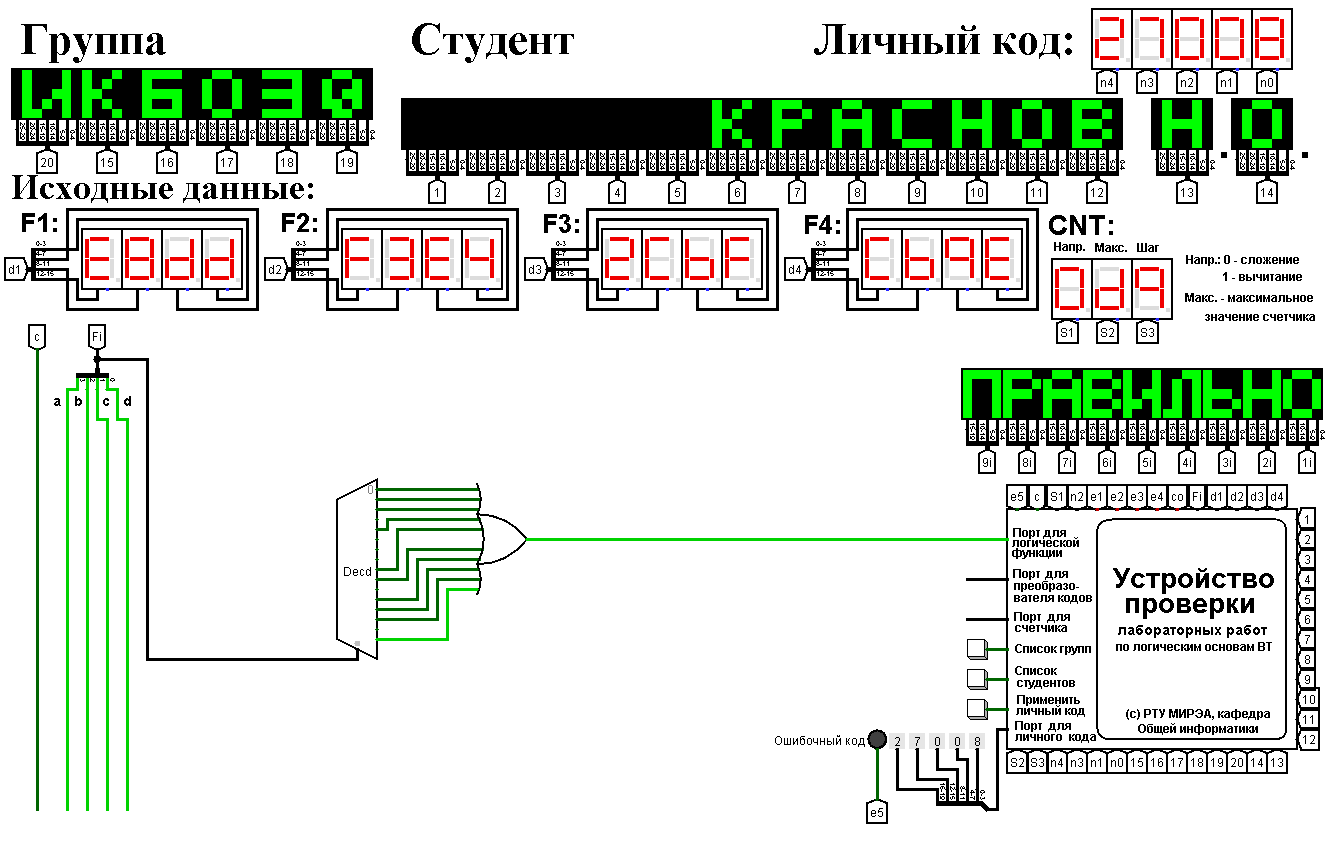
\includegraphics[width=\textwidth]{Дешифр 4-16 ИЛИ.png}
	\caption{Схема, реализующая логическую функцию при помощи дешифратора 4-16}
	\label{fig:Дешифр. 4-16}
\end{figure}

\section{Схема, реализующая логическую функцию при помощи дешифраторов 3-8 и одной дополнительной схемы <<ИЛИ>>}
Реализуем функцию, используя дешифраторы 3-8 и одну дополнительную схему <<ИЛИ>>. Поскольку количество выходов и выходов дешифратора 3-8 меньше количества значений логической функции, нам потребуется распределить области таблицы истинности между двумя дешифраторами, как это показано на таблице \ref{table:Табл. для 3-8}.

\begin{table}[ht]
	\begin{tikzpicture}[remember picture,overlay]
		\foreach \Val in {left,right} {
			\filldraw[
			rounded corners,
			fill=green!30!white,
			draw=black!90!green,
			thick,
			]
			([shift={(-0.1,0.38)}]pic cs:38startgreen\Val) 
			rectangle 
			([shift={(0.1,-0.12)}]pic cs:38endgreen\Val);
		}
		\foreach \Val in {left,right} {
			\filldraw[
			rounded corners,
			fill=red!30!white,
			draw=black!90!red,
			thick,
			]
			([shift={(-0.1,0.38)}]pic cs:38startred\Val) 
			rectangle 
			([shift={(0.1,-0.12)}]pic cs:38endred\Val);
		}

		\node
			(38GL)[text width=4cm] at ([shift={(-3,-1.2)}]pic cs:38startgreenleft)
			{Когда <<a>> равна нулю, работает первый дешифратор};
		\draw
			[-latex,very thick]
			([shift={(0,0.5)}]38GL.south) to [bend right] ([shift={(-0.3,-3.2)}]pic cs:38startgreenleft);
		\node
			(38RL)[text width=4cm] at ([shift={(-3,-1.2)}]pic cs:38startredleft)
			{Когда <<a>> равна единице, работает второй дешифратор};
		\draw
			[-latex,very thick]
			([shift={(0,0.5)}]38RL.south) to [bend right] ([shift={(-0.3,-3.2)}]pic cs:38startredleft);
		\node
			(38GR)[text width=5cm] at ([shift={(6,-1.2)}]pic cs:38startgreenright)
			{Область ответственности первого дешифратора};
		\draw
			[-latex,very thick]
			([shift={(0,0.5)}]38GR.south) to [bend left] ([shift={(0.3,0.4)}]pic cs:38endgreenright);
		\node
			(38RR)[text width=5cm] at ([shift={(6,-1.2)}]pic cs:38startredright)
			{Область ответственности второго дешифратора};
		\draw
			[-latex,very thick]
			([shift={(0,0.5)}]38RR.south) to [bend left] ([shift={(0.3,0.4)}]pic cs:38endredright);
	\end{tikzpicture}
	\centering
	\caption{Распределение областей таблицы истинности между дешифраторами 3-8}
	\label{table:Табл. для 3-8}
	\begin{tabular}{c|c|c|c|c}
		\textbf{a} & \textbf{b} & \textbf{c} & \textbf{d} & \textbf{F} \\
		\hline
		\tikzmark{38startgreenleft}0 & \tikzmark{38startgreenright}0 & 0 & 0 & 1 \\
		\hline
		0 & 0 & 0 & 1 & 1 \\
		\hline
		0 & 0 & 1 & 0 & 1 \\
		\hline
		0 & 0 & 1 & 1 & 0 \\
		\hline
		0 & 1 & 0 & 0 & 1 \\
		\hline
		0 & 1 & 0 & 1 & 0 \\
		\hline
		0 & 1 & 1 & 0 & 0 \\
		\hline
		0\tikzmark{38endgreenleft} & 1 & 1 & 1 & 0\tikzmark{38endgreenright} \\
		\hline
		\tikzmark{38startredleft}1 & \tikzmark{38startredright}0 & 0 & 0 & 1 \\
		\hline
		1 & 0 & 0 & 1 & 1 \\
		\hline
		1 & 0 & 1 & 0 & 0 \\
		\hline
		1 & 0 & 1 & 1 & 1 \\
		\hline
		1 & 1 & 0 & 0 & 1 \\
		\hline
		1 & 1 & 0 & 1 & 1 \\
		\hline
		1 & 1 & 1 & 0 & 0 \\
		\hline
		1\tikzmark{38endredleft} & 1 & 1 & 1 & 1\tikzmark{38endredright} \\
	\end{tabular}
\end{table}

Переменную <<a>> используем для управления дешифраторами. Когда <<a>> равна 0, то должен работать первый дешифратор, который будет отвечать за первую половину таблицы истинности. Когда же <<a>> равна 1, то должен работать второй дешифратор, отвечающий за вторую половину таблицы истинности. Чтобы реализовать это, будем подавать переменную <<a>> на разрешающий вход первого дешифратора через инверсию, а на разрешающий вход второго дешифратора – без инверсии.

В процессе работы на выходах всех дешифраторов будут последовательно появляться единичные значения в соответствии с поступающей на адресные входы комбинаций переменных. Выберем те выходы первого дешифратора, номера которых совпадают с номерами наборов значений переменных, на которых функция равна единице, из первой половины таблицы истинности. У второго дешифратора выберем те входы, номера которых совпадают с номерами наборов значений переменных, на которых функция равна единице, из второй половины таблицы истинности. Объединим выбранные выходы первого и второго дешифратора при помощи схемы «или» и получим требуемую реализацию показанную на рис. \ref{fig:Дешифр. 3-8}.

\begin{figure}[ht]
	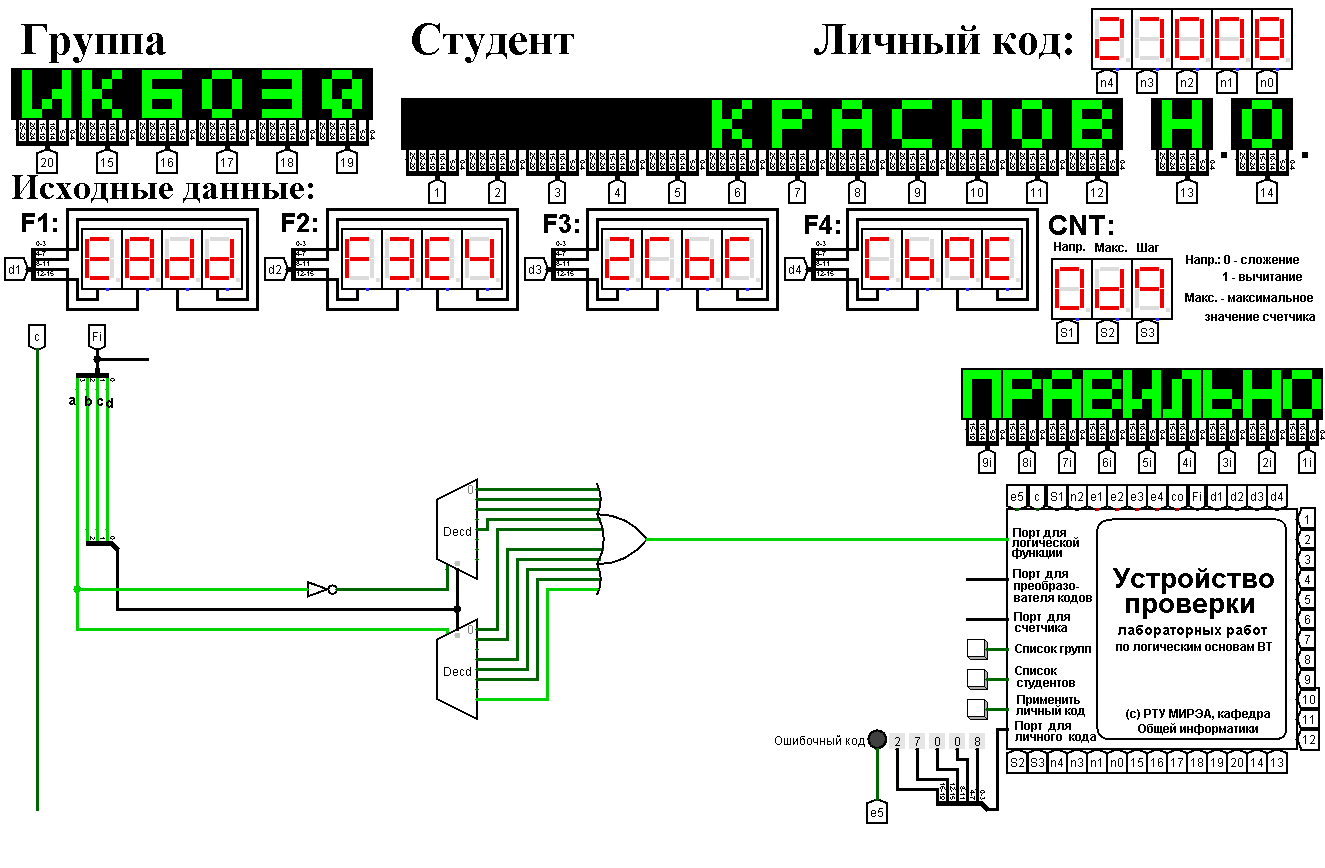
\includegraphics[width=\textwidth]{Дешифр 3-8 ИЛИ.png}
	\caption{Схема, реализующая логическую функцию при помощи дешифраторов 3-8}
	\label{fig:Дешифр. 3-8}
\end{figure}

\section{Схема, реализующая логическую функцию при помощи дешифраторов 2-4 и одной дополнительной схемы <<ИЛИ>>}
Реализуем функцию, используя дешифраторы 2-4 и необходимую дополнительную логику. Поскольку количество выходов и выходов дешифратора 2-4 меньше количества значений логической функции, нам потребуется распределить области таблицы истинности между четырьмя дешифраторами, как это показано на таблице \ref{table:Табл. для 2-4}. Нам потребуется использовать четыре дешифратора 2-4, которые будем называть операционными, и один дешифратор 2-4, который будет управлять первыми четырьмя, назовем его управляющим. Значит, что в общей сложности потребуется пять дешифраторов 2-4 и дополнительная схема <<ИЛИ>>.

\begin{table}[ht]
	\begin{tikzpicture}[remember picture,overlay]
		\foreach \Col in {green,red,blue,yellow} {
			\foreach \Dir in {left,right} {
				\filldraw[
				rounded corners,
				fill=\Col!30!white,
				draw=black!90!\Col,
				thick,
				]
				([shift={(-0.1,0.38)}]pic cs:24start\Col\Dir) 
				rectangle 
				([shift={(0.1,-0.12)}]pic cs:24end\Col\Dir);			
			}
		}
		% ЛЕВАЯ СТОРОНА =============================================
		\node
		(24GL)[outer ysep=1cm,text width=6cm,fill=green!30!white,draw=black!90!green] at ([shift={(-3.5,-0.8)}]pic cs:24startgreenleft)
		{{\small Первый операционный дешифратор включается, когда на адресных входах управляющего дешифратора комбинация 00}};
		\node
		(24RL)[below of=24GL,yshift=-1.5cm,text width=6cm,fill=red!30!white,draw=black!90!red]
		{{\small Второй включается, когда на адресных входах управляющего 01}};
		\node
		(24BL)[below of=24RL,yshift=-1.4cm,text width=6cm,fill=blue!30!white,draw=black!90!blue]
		{{\small Третий включается, когда на адресных входах управляющего 10}};
		\node
		(24YL)[below of=24BL,yshift=-1.4cm,text width=6cm,fill=yellow!30!white,draw=black!90!yellow]
		{{\small Четвертый включается, когда на адресных входах управляющего 11}};
		% ПРАВАЯ СТОРОНА =============================================		
		\node
		(24GR)[outer ysep=1cm,text width=4.7cm,fill=green!30!white,draw=black!90!green] at ([shift={(4.5,-0.8)}]pic cs:24startgreenright)
		{{\small Область ответственности первого операционного дешифратора}};
		\node
		(24RR)[below of=24GR,yshift=-1.4cm,text width=4.7cm,fill=red!30!white,draw=black!90!red]
		{{\small Область ответственности второго операционного дешифратора}};
		\node
		(24BR)[below of=24RR,yshift=-1.4cm,text width=4.7cm,fill=blue!30!white,draw=black!90!blue]
		{{\small Область ответственности третьего операционного дешифратора}};
		\node
		(24YR)[below of=24BR,yshift=-1.4cm,text width=4.7cm,fill=yellow!30!white,draw=black!90!yellow]
		{{\small Область ответственности четвертого операционного дешифратора}};
	\end{tikzpicture}
	\centering
	\caption{Распределение областей таблицы истинности между дешифраторами 2-4}
	\label{table:Табл. для 2-4}
	\begin{tabular}{c|c|c|c|c}
		\textbf{a} & \textbf{b} & \textbf{c} & \textbf{d} & \textbf{F} \\
		\hline
		\tikzmark{24startgreenleft}0 & 0 & \tikzmark{24startgreenright}0 & 0 & 1 \\
		\hline
		0 & 0 & 0 & 1 & 1 \\
		\hline
		0 & 0 & 1 & 0 & 1 \\
		\hline
		0 & 0\tikzmark{24endgreenleft} & 1 & 1 & 0\tikzmark{24endgreenright} \\
		\hline
		\tikzmark{24startredleft}0 & 1 & \tikzmark{24startredright}0 & 0 & 1 \\
		\hline
		0 & 1 & 0 & 1 & 0 \\
		\hline
		0 & 1 & 1 & 0 & 0 \\
		\hline
		0 & 1\tikzmark{24endredleft} & 1 & 1 & 0\tikzmark{24endredright} \\
		\hline
		\tikzmark{24startblueleft}1 & 0 & \tikzmark{24startblueright}0 & 0 & 1 \\
		\hline
		1 & 0 & 0 & 1 & 1 \\
		\hline
		1 & 0 & 1 & 0 & 0 \\
		\hline
		1 & 0\tikzmark{24endblueleft} & 1 & 1 & 1\tikzmark{24endblueright} \\
		\hline
		\tikzmark{24startyellowleft}1 & 1 & \tikzmark{24startyellowright}0 & 0 & 1 \\
		\hline
		1 & 1 & 0 & 1 & 1 \\
		\hline
		1 & 1 & 1 & 0 & 0 \\
		\hline
		1 & 1\tikzmark{24endyellowleft} & 1 & 1 & 1\tikzmark{24endyellowright} \\
	\end{tabular}
\end{table}

Теперь каждый операционный дешифратор отвечает за свою двоичную тетраду в исходной векторной записи логической функции. Выберем у каждого операционного дешифратора те выходы, где у двоичной тетрады стоят единицы, причем будем считать, что нулевой выход дешифратора соответствует старшему двоичному разряду тетрады. Объединим выбранные выходы при помощи схемы <<ИЛИ>>, и получим требуемую реализацию (рис. \ref{fig:Дешифр. 2-4}).

\begin{figure}[ht]
	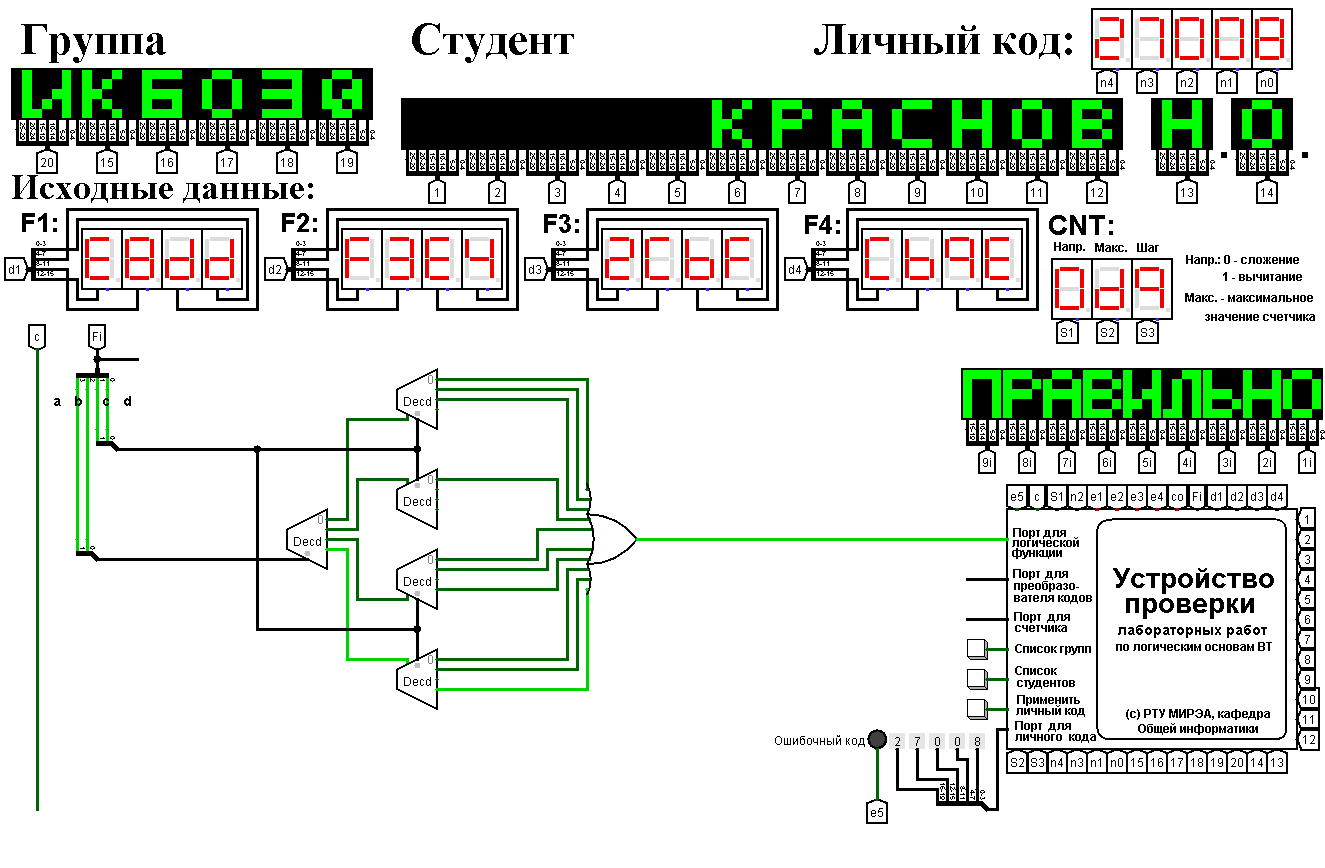
\includegraphics[width=\textwidth]{Дешифр 2-4 ИЛИ.png}
	\caption{Схема, реализующая логическую функцию при помощи дешифраторов 2-4}
	\label{fig:Дешифр. 2-4}
\end{figure}

\chapter{ВЫВОДЫ}
В этой практической работе были освоены навыки построения комбинационных схем, реализующих логическую функцию на дешифраторах 4-16, 3-8 и 2-4 в среде схемотехнического моделирования Logisim, используя необходимую дополнительную логику и один дополнительный элемент <<ИЛИ>>.

\begin{thebibliography}{99}
	\bibitem{Методичка} \textbf{Смирнов, С.С.} Информатика. Методические указания по выполнению практических работ / С.С. Смирнов, Д.А. Карпов. – Москва, МИРЭА – Российский технологический университет, 2020. – 102 с.
	
	\bibitem{Logisim} Logisim / разработчик: Карл Берч. – 2014. – URL: http://www.cburch.com/logisim/index.html (дата обращения 26.10.2022). – версия 2.7.0 . – Электронная программа : электронная.
\end{thebibliography}


\end{document}
